\documentclass[1p]{elsarticle_modified}
%\bibliographystyle{elsarticle-num}

%\usepackage[colorlinks]{hyperref}
%\usepackage{abbrmath_seonhwa} %\Abb, \Ascr, \Acal ,\Abf, \Afrak
\usepackage{amsfonts}
\usepackage{amssymb}
\usepackage{amsmath}
\usepackage{amsthm}
\usepackage{scalefnt}
\usepackage{amsbsy}
\usepackage{kotex}
\usepackage{caption}
\usepackage{subfig}
\usepackage{color}
\usepackage{graphicx}
\usepackage{xcolor} %% white, black, red, green, blue, cyan, magenta, yellow
\usepackage{float}
\usepackage{setspace}
\usepackage{hyperref}

\usepackage{tikz}
\usetikzlibrary{arrows}

\usepackage{multirow}
\usepackage{array} % fixed length table
\usepackage{hhline}

%%%%%%%%%%%%%%%%%%%%%
\makeatletter
\renewcommand*\env@matrix[1][\arraystretch]{%
	\edef\arraystretch{#1}%
	\hskip -\arraycolsep
	\let\@ifnextchar\new@ifnextchar
	\array{*\c@MaxMatrixCols c}}
\makeatother %https://tex.stackexchange.com/questions/14071/how-can-i-increase-the-line-spacing-in-a-matrix
%%%%%%%%%%%%%%%

\usepackage[normalem]{ulem}

\newcommand{\msout}[1]{\ifmmode\text{\sout{\ensuremath{#1}}}\else\sout{#1}\fi}
%SOURCE: \msout is \stkout macro in https://tex.stackexchange.com/questions/20609/strikeout-in-math-mode

\newcommand{\cancel}[1]{
	\ifmmode
	{\color{red}\msout{#1}}
	\else
	{\color{red}\sout{#1}}
	\fi
}

\newcommand{\add}[1]{
	{\color{blue}\uwave{#1}}
}

\newcommand{\replace}[2]{
	\ifmmode
	{\color{red}\msout{#1}}{\color{blue}\uwave{#2}}
	\else
	{\color{red}\sout{#1}}{\color{blue}\uwave{#2}}
	\fi
}

\newcommand{\Sol}{\mathcal{S}} %segment
\newcommand{\D}{D} %diagram
\newcommand{\A}{\mathcal{A}} %arc


%%%%%%%%%%%%%%%%%%%%%%%%%%%%%5 test

\def\sl{\operatorname{\textup{SL}}(2,\Cbb)}
\def\psl{\operatorname{\textup{PSL}}(2,\Cbb)}
\def\quan{\mkern 1mu \triangleright \mkern 1mu}

\theoremstyle{definition}
\newtheorem{thm}{Theorem}[section]
\newtheorem{prop}[thm]{Proposition}
\newtheorem{lem}[thm]{Lemma}
\newtheorem{ques}[thm]{Question}
\newtheorem{cor}[thm]{Corollary}
\newtheorem{defn}[thm]{Definition}
\newtheorem{exam}[thm]{Example}
\newtheorem{rmk}[thm]{Remark}
\newtheorem{alg}[thm]{Algorithm}

\newcommand{\I}{\sqrt{-1}}
\begin{document}

%\begin{frontmatter}
%
%\title{Boundary parabolic representations of knots up to 8 crossings}
%
%%% Group authors per affiliation:
%\author{Yunhi Cho} 
%\address{Department of Mathematics, University of Seoul, Seoul, Korea}
%\ead{yhcho@uos.ac.kr}
%
%
%\author{Seonhwa Kim} %\fnref{s_kim}}
%\address{Center for Geometry and Physics, Institute for Basic Science, Pohang, 37673, Korea}
%\ead{ryeona17@ibs.re.kr}
%
%\author{Hyuk Kim}
%\address{Department of Mathematical Sciences, Seoul National University, Seoul 08826, Korea}
%\ead{hyukkim@snu.ac.kr}
%
%\author{Seokbeom Yoon}
%\address{Department of Mathematical Sciences, Seoul National University, Seoul, 08826,  Korea}
%\ead{sbyoon15@snu.ac.kr}
%
%\begin{abstract}
%We find all boundary parabolic representation of knots up to 8 crossings.
%
%\end{abstract}
%\begin{keyword}
%    \MSC[2010] 57M25 
%\end{keyword}
%
%\end{frontmatter}

%\linenumbers
%\tableofcontents
%
\newcommand\colored[1]{\textcolor{white}{\rule[-0.35ex]{0.8em}{1.4ex}}\kern-0.8em\color{red} #1}%
%\newcommand\colored[1]{\textcolor{white}{ #1}\kern-2.17ex	\textcolor{white}{ #1}\kern-1.81ex	\textcolor{white}{ #1}\kern-2.15ex\color{red}#1	}

{\Large $\underline{12n_{0043}~(K12n_{0043})}$}

\setlength{\tabcolsep}{10pt}
\renewcommand{\arraystretch}{1.6}
\vspace{1cm}\begin{tabular}{m{100pt}>{\centering\arraybackslash}m{274pt}}
\multirow{5}{120pt}{
	\centering
	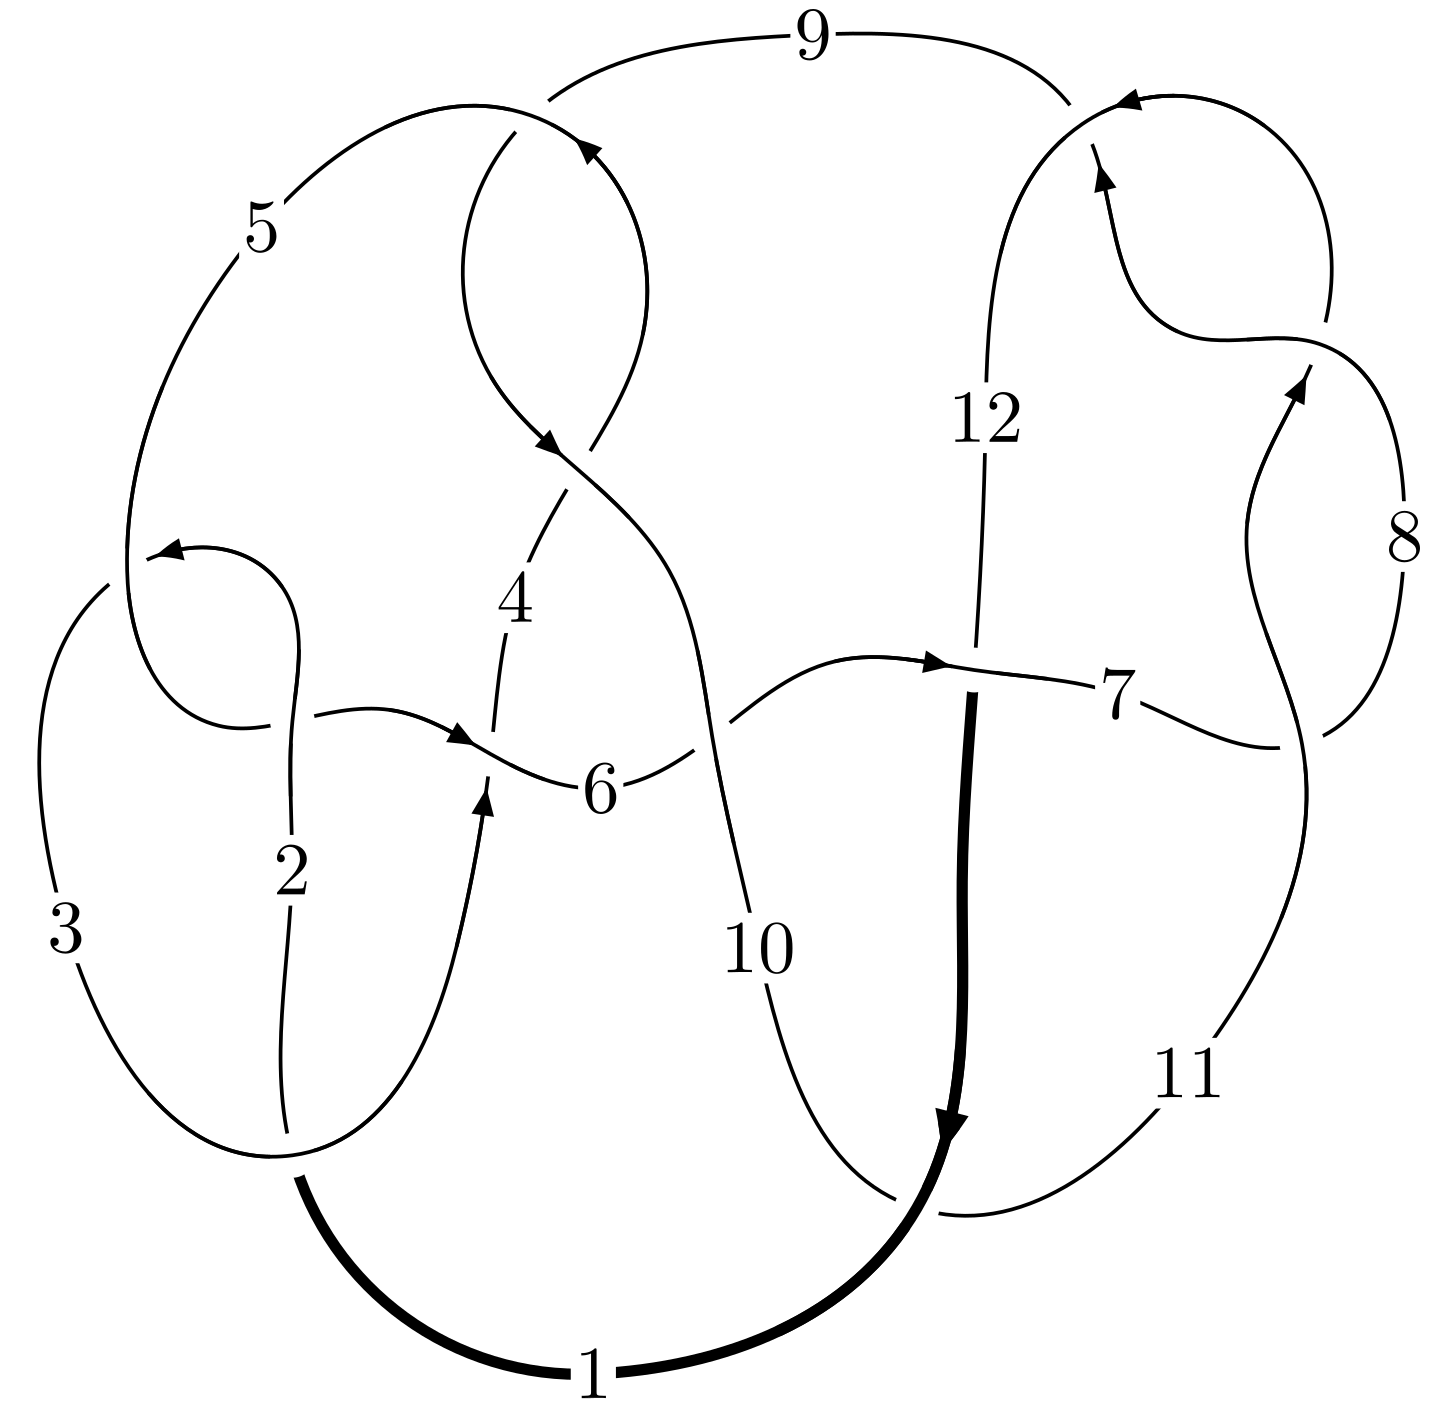
\includegraphics[width=112pt]{../../../GIT/diagram.site/Diagrams/png/2132_12n_0043.png}\\
\ \ \ A knot diagram\footnotemark}&
\allowdisplaybreaks
\textbf{Linearized knot diagam} \\
\cline{2-2}
 &
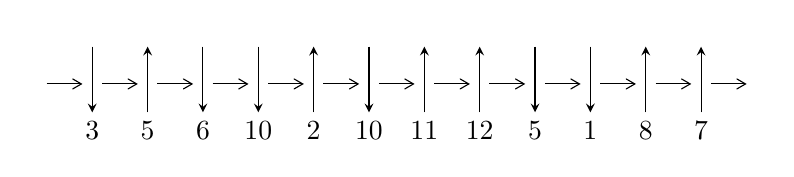
\begin{tikzpicture}[x=20pt, y=17pt]
	% nodes
	\node (C0) at (0, 0) {};
	\node (C1) at (1, 0) {};
	\node (C1U) at (1, +1) {};
	\node (C1D) at (1, -1) {3};

	\node (C2) at (2, 0) {};
	\node (C2U) at (2, +1) {};
	\node (C2D) at (2, -1) {5};

	\node (C3) at (3, 0) {};
	\node (C3U) at (3, +1) {};
	\node (C3D) at (3, -1) {6};

	\node (C4) at (4, 0) {};
	\node (C4U) at (4, +1) {};
	\node (C4D) at (4, -1) {10};

	\node (C5) at (5, 0) {};
	\node (C5U) at (5, +1) {};
	\node (C5D) at (5, -1) {2};

	\node (C6) at (6, 0) {};
	\node (C6U) at (6, +1) {};
	\node (C6D) at (6, -1) {10};

	\node (C7) at (7, 0) {};
	\node (C7U) at (7, +1) {};
	\node (C7D) at (7, -1) {11};

	\node (C8) at (8, 0) {};
	\node (C8U) at (8, +1) {};
	\node (C8D) at (8, -1) {12};

	\node (C9) at (9, 0) {};
	\node (C9U) at (9, +1) {};
	\node (C9D) at (9, -1) {5};

	\node (C10) at (10, 0) {};
	\node (C10U) at (10, +1) {};
	\node (C10D) at (10, -1) {1};

	\node (C11) at (11, 0) {};
	\node (C11U) at (11, +1) {};
	\node (C11D) at (11, -1) {8};

	\node (C12) at (12, 0) {};
	\node (C12U) at (12, +1) {};
	\node (C12D) at (12, -1) {7};
	\node (C13) at (13, 0) {};

	% arrows
	\draw[->,>={angle 60}]
	(C0) edge (C1) (C1) edge (C2) (C2) edge (C3) (C3) edge (C4) (C4) edge (C5) (C5) edge (C6) (C6) edge (C7) (C7) edge (C8) (C8) edge (C9) (C9) edge (C10) (C10) edge (C11) (C11) edge (C12) (C12) edge (C13) ;	\draw[->,>=stealth]
	(C1U) edge (C1D) (C2D) edge (C2U) (C3U) edge (C3D) (C4U) edge (C4D) (C5D) edge (C5U) (C6U) edge (C6D) (C7D) edge (C7U) (C8D) edge (C8U) (C9U) edge (C9D) (C10U) edge (C10D) (C11D) edge (C11U) (C12D) edge (C12U) ;
	\end{tikzpicture} \\
\hhline{~~} \\& 
\textbf{Solving Sequence} \\ \cline{2-2} 
 &
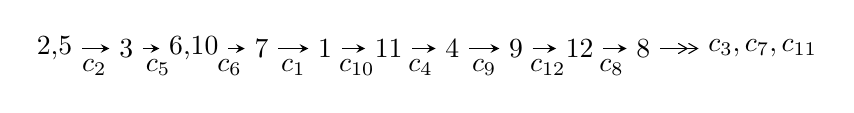
\begin{tikzpicture}[x=23pt, y=7pt]
	% node
	\node (A0) at (-1/8, 0) {2,5};
	\node (A1) at (1, 0) {3};
	\node (A2) at (33/16, 0) {6,10};
	\node (A3) at (25/8, 0) {7};
	\node (A4) at (33/8, 0) {1};
	\node (A5) at (41/8, 0) {11};
	\node (A6) at (49/8, 0) {4};
	\node (A7) at (57/8, 0) {9};
	\node (A8) at (65/8, 0) {12};
	\node (A9) at (73/8, 0) {8};
	\node (C1) at (1/2, -1) {$c_{2}$};
	\node (C2) at (3/2, -1) {$c_{5}$};
	\node (C3) at (21/8, -1) {$c_{6}$};
	\node (C4) at (29/8, -1) {$c_{1}$};
	\node (C5) at (37/8, -1) {$c_{10}$};
	\node (C6) at (45/8, -1) {$c_{4}$};
	\node (C7) at (53/8, -1) {$c_{9}$};
	\node (C8) at (61/8, -1) {$c_{12}$};
	\node (C9) at (69/8, -1) {$c_{8}$};
	\node (A10) at (11, 0) {$c_{3},c_{7},c_{11}$};

	% edge
	\draw[->,>=stealth]	
	(A0) edge (A1) (A1) edge (A2) (A2) edge (A3) (A3) edge (A4) (A4) edge (A5) (A5) edge (A6) (A6) edge (A7) (A7) edge (A8) (A8) edge (A9) ;
	\draw[->>,>={angle 60}]	
	(A9) edge (A10);
\end{tikzpicture} \\ 

\end{tabular} \\

\footnotetext{
The image of knot diagram is generated by the software ``\textbf{Draw programme}" developed by Andrew Bartholomew(\url{http://www.layer8.co.uk/maths/draw/index.htm\#Running-draw}), where we modified some parts for our purpose(\url{https://github.com/CATsTAILs/LinksPainter}).
}\phantom \\ \newline 
\centering \textbf{Ideals for irreducible components\footnotemark of $X_{\text{par}}$} 
 
\begin{align*}
I^u_{1}&=\langle 
15 u^{49}-122 u^{48}+\cdots+16 b-5,\;6 u^{49}-51 u^{48}+\cdots+8 a-7,\;u^{50}-6 u^{49}+\cdots-3 u+1\rangle \\
I^u_{2}&=\langle 
b^5- b^4 u- b^4+2 b^3 u+b^2- b u- b+u,\;a,\;u^2+u+1\rangle \\
\\
\end{align*}
\raggedright * 2 irreducible components of $\dim_{\mathbb{C}}=0$, with total 60 representations.\\
\footnotetext{All coefficients of polynomials are rational numbers. But the coefficients are sometimes approximated in decimal forms when there is not enough margin.}
\newpage
\renewcommand{\arraystretch}{1}
\centering \section*{I. $I^u_{1}= \langle 15 u^{49}-122 u^{48}+\cdots+16 b-5,\;6 u^{49}-51 u^{48}+\cdots+8 a-7,\;u^{50}-6 u^{49}+\cdots-3 u+1 \rangle$}
\flushleft \textbf{(i) Arc colorings}\\
\begin{tabular}{m{7pt} m{180pt} m{7pt} m{180pt} }
\flushright $a_{2}=$&$\begin{pmatrix}1\\0\end{pmatrix}$ \\
\flushright $a_{5}=$&$\begin{pmatrix}0\\u\end{pmatrix}$ \\
\flushright $a_{3}=$&$\begin{pmatrix}1\\- u^2\end{pmatrix}$ \\
\flushright $a_{6}=$&$\begin{pmatrix}u\\u\end{pmatrix}$ \\
\flushright $a_{10}=$&$\begin{pmatrix}-\frac{3}{4} u^{49}+\frac{51}{8} u^{48}+\cdots-\frac{3}{2} u+\frac{7}{8}\\-0.937500 u^{49}+7.62500 u^{48}+\cdots-1.68750 u+0.312500\end{pmatrix}$ \\
\flushright $a_{7}=$&$\begin{pmatrix}- u^2-1\\-0.0625000 u^{48}+0.312500 u^{47}+\cdots+2.12500 u-0.0625000\end{pmatrix}$ \\
\flushright $a_{1}=$&$\begin{pmatrix}u^2+1\\- u^4\end{pmatrix}$ \\
\flushright $a_{11}=$&$\begin{pmatrix}-2.81250 u^{49}+17.4375 u^{48}+\cdots-6.56250 u+2.75000\\-3.75000 u^{49}+23.4375 u^{48}+\cdots-6.50000 u+1.18750\end{pmatrix}$ \\
\flushright $a_{4}=$&$\begin{pmatrix}u^4+u^2+1\\u^4\end{pmatrix}$ \\
\flushright $a_{9}=$&$\begin{pmatrix}-\frac{3}{4} u^{49}+\frac{51}{8} u^{48}+\cdots-\frac{3}{2} u+\frac{7}{8}\\-1.81250 u^{49}+14.8750 u^{48}+\cdots-8.06250 u+2.18750\end{pmatrix}$ \\
\flushright $a_{12}=$&$\begin{pmatrix}\frac{1}{16} u^{49}-\frac{3}{8} u^{48}+\cdots-\frac{29}{16} u+\frac{15}{16}\\\frac{5}{8} u^{49}-\frac{19}{8} u^{48}+\cdots-\frac{9}{8} u+\frac{7}{8}\end{pmatrix}$ \\
\flushright $a_{8}=$&$\begin{pmatrix}\frac{1}{2} u^{49}-\frac{53}{16} u^{48}+\cdots+\frac{25}{4} u-\frac{13}{16}\\-0.187500 u^{49}-0.687500 u^{48}+\cdots+4.43750 u-1.75000\end{pmatrix}$\\&\end{tabular}
\flushleft \textbf{(ii) Obstruction class $= -1$}\\~\\
\flushleft \textbf{(iii) Cusp Shapes $= -\frac{235}{16} u^{49}+\frac{1341}{16} u^{48}+\cdots-\frac{101}{16} u-\frac{1}{2}$}\\~\\
\newpage\renewcommand{\arraystretch}{1}
\flushleft \textbf{(iv) u-Polynomials at the component}\newline \\
\begin{tabular}{m{50pt}|m{274pt}}
Crossings & \hspace{64pt}u-Polynomials at each crossing \\
\hline $$\begin{aligned}c_{1}\end{aligned}$$&$\begin{aligned}
&u^{50}+30 u^{49}+\cdots+9 u+1
\end{aligned}$\\
\hline $$\begin{aligned}c_{2},c_{5}\end{aligned}$$&$\begin{aligned}
&u^{50}+6 u^{49}+\cdots+3 u+1
\end{aligned}$\\
\hline $$\begin{aligned}c_{3}\end{aligned}$$&$\begin{aligned}
&u^{50}-6 u^{49}+\cdots-5 u+2
\end{aligned}$\\
\hline $$\begin{aligned}c_{4},c_{9}\end{aligned}$$&$\begin{aligned}
&u^{50}- u^{49}+\cdots+1024 u+1024
\end{aligned}$\\
\hline $$\begin{aligned}c_{6}\end{aligned}$$&$\begin{aligned}
&u^{50}+3 u^{49}+\cdots+9 u^2+1
\end{aligned}$\\
\hline $$\begin{aligned}c_{7},c_{8},c_{11}\end{aligned}$$&$\begin{aligned}
&u^{50}-3 u^{49}+\cdots+9 u^2+1
\end{aligned}$\\
\hline $$\begin{aligned}c_{10}\end{aligned}$$&$\begin{aligned}
&u^{50}-13 u^{49}+\cdots-146 u-7
\end{aligned}$\\
\hline $$\begin{aligned}c_{12}\end{aligned}$$&$\begin{aligned}
&u^{50}+9 u^{49}+\cdots+227 u+32
\end{aligned}$\\
\hline
\end{tabular}\\~\\
\newpage\renewcommand{\arraystretch}{1}
\flushleft \textbf{(v) Riley Polynomials at the component}\newline \\
\begin{tabular}{m{50pt}|m{274pt}}
Crossings & \hspace{64pt}Riley Polynomials at each crossing \\
\hline $$\begin{aligned}c_{1}\end{aligned}$$&$\begin{aligned}
&y^{50}-14 y^{49}+\cdots+9 y+1
\end{aligned}$\\
\hline $$\begin{aligned}c_{2},c_{5}\end{aligned}$$&$\begin{aligned}
&y^{50}+30 y^{49}+\cdots+9 y+1
\end{aligned}$\\
\hline $$\begin{aligned}c_{3}\end{aligned}$$&$\begin{aligned}
&y^{50}-58 y^{49}+\cdots+63 y+4
\end{aligned}$\\
\hline $$\begin{aligned}c_{4},c_{9}\end{aligned}$$&$\begin{aligned}
&y^{50}-55 y^{49}+\cdots-12582912 y+1048576
\end{aligned}$\\
\hline $$\begin{aligned}c_{6}\end{aligned}$$&$\begin{aligned}
&y^{50}-61 y^{49}+\cdots+18 y+1
\end{aligned}$\\
\hline $$\begin{aligned}c_{7},c_{8},c_{11}\end{aligned}$$&$\begin{aligned}
&y^{50}-45 y^{49}+\cdots+18 y+1
\end{aligned}$\\
\hline $$\begin{aligned}c_{10}\end{aligned}$$&$\begin{aligned}
&y^{50}- y^{49}+\cdots-19146 y+49
\end{aligned}$\\
\hline $$\begin{aligned}c_{12}\end{aligned}$$&$\begin{aligned}
&y^{50}+7 y^{49}+\cdots+13303 y+1024
\end{aligned}$\\
\hline
\end{tabular}\\~\\
\newpage\flushleft \textbf{(vi) Complex Volumes and Cusp Shapes}
$$\begin{array}{c|c|c}  
\text{Solutions to }I^u_{1}& \I (\text{vol} + \sqrt{-1}CS) & \text{Cusp shape}\\
 \hline 
\begin{aligned}
u &= \phantom{-}0.973341 + 0.149524 I \\
a &= -1.68794 - 0.12351 I \\
b &= \phantom{-}0.066174 - 0.254632 I\end{aligned}
 & -1.48997 - 8.27576 I & \phantom{-}2.25055 + 4.63368 I \\ \hline\begin{aligned}
u &= \phantom{-}0.973341 - 0.149524 I \\
a &= -1.68794 + 0.12351 I \\
b &= \phantom{-}0.066174 + 0.254632 I\end{aligned}
 & -1.48997 + 8.27576 I & \phantom{-}2.25055 - 4.63368 I \\ \hline\begin{aligned}
u &= \phantom{-}0.973094 + 0.107852 I \\
a &= \phantom{-}1.69811 + 0.08847 I \\
b &= -0.056748 + 0.182641 I\end{aligned}
 & -6.65156 - 4.37591 I & -2.22838 + 3.56988 I \\ \hline\begin{aligned}
u &= \phantom{-}0.973094 - 0.107852 I \\
a &= \phantom{-}1.69811 - 0.08847 I \\
b &= -0.056748 - 0.182641 I\end{aligned}
 & -6.65156 + 4.37591 I & -2.22838 - 3.56988 I \\ \hline\begin{aligned}
u &= -0.677365 + 0.699027 I \\
a &= -0.322440 - 0.902269 I \\
b &= -0.498316 - 0.530339 I\end{aligned}
 & \phantom{-}4.64833 + 0.74609 I & \phantom{-}3.29001 + 0. I\phantom{ +0.000000I} \\ \hline\begin{aligned}
u &= -0.677365 - 0.699027 I \\
a &= -0.322440 + 0.902269 I \\
b &= -0.498316 + 0.530339 I\end{aligned}
 & \phantom{-}4.64833 - 0.74609 I & \phantom{-}3.29001 + 0. I\phantom{ +0.000000I} \\ \hline\begin{aligned}
u &= \phantom{-}0.957021 + 0.043611 I \\
a &= -1.69470 - 0.03418 I \\
b &= \phantom{-}0.0746266 - 0.0721643 I\end{aligned}
 & -4.57488 - 0.26600 I & \phantom{-0.000000 }      -6
0. 10   - 1.059498 I \\ \hline\begin{aligned}
u &= \phantom{-}0.957021 - 0.043611 I \\
a &= -1.69470 + 0.03418 I \\
b &= \phantom{-}0.0746266 + 0.0721643 I\end{aligned}
 & -4.57488 + 0.26600 I & \phantom{-0.000000 -}     -6
0. 10   + 1.059498 I \\ \hline\begin{aligned}
u &= \phantom{-}0.236301 + 0.909169 I \\
a &= -0.572242 + 0.629406 I \\
b &= \phantom{-}0.72257 + 1.84188 I\end{aligned}
 & \phantom{-}5.03527 + 5.79377 I & -0.60515 - 2.37720 I \\ \hline\begin{aligned}
u &= \phantom{-}0.236301 - 0.909169 I \\
a &= -0.572242 - 0.629406 I \\
b &= \phantom{-}0.72257 - 1.84188 I\end{aligned}
 & \phantom{-}5.03527 - 5.79377 I & -0.60515 + 2.37720 I\\
 \hline 
 \end{array}$$\newpage$$\begin{array}{c|c|c}  
\text{Solutions to }I^u_{1}& \I (\text{vol} + \sqrt{-1}CS) & \text{Cusp shape}\\
 \hline 
\begin{aligned}
u &= \phantom{-}0.161591 + 0.918734 I \\
a &= \phantom{-}0.626446 - 0.670903 I \\
b &= -0.48442 - 1.64182 I\end{aligned}
 & -0.70904 + 2.61756 I & -4.03413 - 3.04976 I \\ \hline\begin{aligned}
u &= \phantom{-}0.161591 - 0.918734 I \\
a &= \phantom{-}0.626446 + 0.670903 I \\
b &= -0.48442 + 1.64182 I\end{aligned}
 & -0.70904 - 2.61756 I & -4.03413 + 3.04976 I \\ \hline\begin{aligned}
u &= -0.502925 + 0.747274 I \\
a &= -0.018799 + 0.638607 I \\
b &= \phantom{-}0.247387 + 0.438501 I\end{aligned}
 & \phantom{-}0.02112 - 1.45050 I & -2.86693 + 5.13818 I \\ \hline\begin{aligned}
u &= -0.502925 - 0.747274 I \\
a &= -0.018799 - 0.638607 I \\
b &= \phantom{-}0.247387 - 0.438501 I\end{aligned}
 & \phantom{-}0.02112 + 1.45050 I & -2.86693 - 5.13818 I \\ \hline\begin{aligned}
u &= -0.609640 + 0.928743 I \\
a &= -0.602842 - 0.340623 I \\
b &= -0.607870 - 0.045415 I\end{aligned}
 & -0.64445 - 3.09089 I & \phantom{-0.000000 } 0 \\ \hline\begin{aligned}
u &= -0.609640 - 0.928743 I \\
a &= -0.602842 + 0.340623 I \\
b &= -0.607870 + 0.045415 I\end{aligned}
 & -0.64445 + 3.09089 I & \phantom{-0.000000 } 0 \\ \hline\begin{aligned}
u &= -0.115719 + 1.106410 I \\
a &= -0.816238 + 0.672347 I \\
b &= -0.366736 + 1.302780 I\end{aligned}
 & -0.489731 + 0.237177 I & \phantom{-0.000000 } 0 \\ \hline\begin{aligned}
u &= -0.115719 - 1.106410 I \\
a &= -0.816238 - 0.672347 I \\
b &= -0.366736 - 1.302780 I\end{aligned}
 & -0.489731 - 0.237177 I & \phantom{-0.000000 } 0 \\ \hline\begin{aligned}
u &= -0.686560 + 0.915627 I \\
a &= \phantom{-}0.693027 + 0.536546 I \\
b &= \phantom{-}0.731923 + 0.193983 I\end{aligned}
 & \phantom{-}4.03197 - 5.98158 I & \phantom{-0.000000 } 0 \\ \hline\begin{aligned}
u &= -0.686560 - 0.915627 I \\
a &= \phantom{-}0.693027 - 0.536546 I \\
b &= \phantom{-}0.731923 - 0.193983 I\end{aligned}
 & \phantom{-}4.03197 + 5.98158 I & \phantom{-0.000000 } 0\\
 \hline 
 \end{array}$$\newpage$$\begin{array}{c|c|c}  
\text{Solutions to }I^u_{1}& \I (\text{vol} + \sqrt{-1}CS) & \text{Cusp shape}\\
 \hline 
\begin{aligned}
u &= -0.243021 + 1.135140 I \\
a &= \phantom{-}0.892386 - 0.542794 I \\
b &= \phantom{-}0.566389 - 1.069200 I\end{aligned}
 & -3.49782 - 3.09462 I & \phantom{-0.000000 } 0 \\ \hline\begin{aligned}
u &= -0.243021 - 1.135140 I \\
a &= \phantom{-}0.892386 + 0.542794 I \\
b &= \phantom{-}0.566389 + 1.069200 I\end{aligned}
 & -3.49782 + 3.09462 I & \phantom{-0.000000 } 0 \\ \hline\begin{aligned}
u &= -0.538980 + 1.033550 I \\
a &= \phantom{-}0.798066 + 0.043574 I \\
b &= \phantom{-}0.699077 - 0.292935 I\end{aligned}
 & \phantom{-}2.94116 - 0.76505 I & \phantom{-0.000000 } 0 \\ \hline\begin{aligned}
u &= -0.538980 - 1.033550 I \\
a &= \phantom{-}0.798066 - 0.043574 I \\
b &= \phantom{-}0.699077 + 0.292935 I\end{aligned}
 & \phantom{-}2.94116 + 0.76505 I & \phantom{-0.000000 } 0 \\ \hline\begin{aligned}
u &= \phantom{-}0.022608 + 0.789395 I \\
a &= -0.701358 + 0.689418 I \\
b &= \phantom{-}0.406014 + 1.098740 I\end{aligned}
 & -0.100668 - 0.941081 I & -0.92280 + 4.24243 I \\ \hline\begin{aligned}
u &= \phantom{-}0.022608 - 0.789395 I \\
a &= -0.701358 - 0.689418 I \\
b &= \phantom{-}0.406014 - 1.098740 I\end{aligned}
 & -0.100668 + 0.941081 I & -0.92280 - 4.24243 I \\ \hline\begin{aligned}
u &= -0.311220 + 1.172780 I \\
a &= -0.971626 + 0.461124 I \\
b &= -0.720591 + 0.967453 I\end{aligned}
 & \phantom{-}1.10315 - 6.57415 I & \phantom{-0.000000 } 0 \\ \hline\begin{aligned}
u &= -0.311220 - 1.172780 I \\
a &= -0.971626 - 0.461124 I \\
b &= -0.720591 - 0.967453 I\end{aligned}
 & \phantom{-}1.10315 + 6.57415 I & \phantom{-0.000000 } 0 \\ \hline\begin{aligned}
u &= \phantom{-}0.778276\phantom{ +0.000000I} \\
a &= \phantom{-}1.59204\phantom{ +0.000000I} \\
b &= -0.332020\phantom{ +0.000000I}\end{aligned}
 & \phantom{-}2.53130\phantom{ +0.000000I} & \phantom{-}4.52920\phantom{ +0.000000I} \\ \hline\begin{aligned}
u &= \phantom{-}0.215175 + 0.693272 I \\
a &= \phantom{-}0.787829 - 0.545376 I \\
b &= -0.975052 - 0.975693 I\end{aligned}
 & \phantom{-}5.65570 - 3.38770 I & \phantom{-}2.66671 + 5.35428 I\\
 \hline 
 \end{array}$$\newpage$$\begin{array}{c|c|c}  
\text{Solutions to }I^u_{1}& \I (\text{vol} + \sqrt{-1}CS) & \text{Cusp shape}\\
 \hline 
\begin{aligned}
u &= \phantom{-}0.215175 - 0.693272 I \\
a &= \phantom{-}0.787829 + 0.545376 I \\
b &= -0.975052 + 0.975693 I\end{aligned}
 & \phantom{-}5.65570 + 3.38770 I & \phantom{-}2.66671 - 5.35428 I \\ \hline\begin{aligned}
u &= \phantom{-}0.476948 + 1.225580 I \\
a &= -0.211170 + 1.154370 I \\
b &= -0.37574 + 2.70281 I\end{aligned}
 & -0.98640 + 4.59430 I & \phantom{-0.000000 } 0 \\ \hline\begin{aligned}
u &= \phantom{-}0.476948 - 1.225580 I \\
a &= -0.211170 - 1.154370 I \\
b &= -0.37574 - 2.70281 I\end{aligned}
 & -0.98640 - 4.59430 I & \phantom{-0.000000 } 0 \\ \hline\begin{aligned}
u &= \phantom{-}0.510209 + 1.283800 I \\
a &= \phantom{-}0.195449 - 1.284720 I \\
b &= \phantom{-}0.45463 - 2.70776 I\end{aligned}
 & -8.38002 + 5.49910 I & \phantom{-0.000000 } 0 \\ \hline\begin{aligned}
u &= \phantom{-}0.510209 - 1.283800 I \\
a &= \phantom{-}0.195449 + 1.284720 I \\
b &= \phantom{-}0.45463 + 2.70776 I\end{aligned}
 & -8.38002 - 5.49910 I & \phantom{-0.000000 } 0 \\ \hline\begin{aligned}
u &= -0.565504 + 0.246324 I \\
a &= \phantom{-}0.06152 - 1.46066 I \\
b &= -0.182316 - 0.730281 I\end{aligned}
 & \phantom{-}4.93756 - 3.55579 I & \phantom{-}5.87055 + 4.25691 I \\ \hline\begin{aligned}
u &= -0.565504 - 0.246324 I \\
a &= \phantom{-}0.06152 + 1.46066 I \\
b &= -0.182316 + 0.730281 I\end{aligned}
 & \phantom{-}4.93756 + 3.55579 I & \phantom{-}5.87055 - 4.25691 I \\ \hline\begin{aligned}
u &= \phantom{-}0.562121 + 1.266420 I \\
a &= \phantom{-}0.086370 - 1.295980 I \\
b &= \phantom{-}0.45752 - 2.75201 I\end{aligned}
 & -4.9120 + 13.8047 I & \phantom{-0.000000 } 0 \\ \hline\begin{aligned}
u &= \phantom{-}0.562121 - 1.266420 I \\
a &= \phantom{-}0.086370 + 1.295980 I \\
b &= \phantom{-}0.45752 + 2.75201 I\end{aligned}
 & -4.9120 - 13.8047 I & \phantom{-0.000000 } 0 \\ \hline\begin{aligned}
u &= \phantom{-}0.383593 + 1.332350 I \\
a &= \phantom{-}0.449050 - 1.266840 I \\
b &= \phantom{-}0.50380 - 2.53593 I\end{aligned}
 & -6.24884 - 3.57394 I & \phantom{-0.000000 } 0\\
 \hline 
 \end{array}$$\newpage$$\begin{array}{c|c|c}  
\text{Solutions to }I^u_{1}& \I (\text{vol} + \sqrt{-1}CS) & \text{Cusp shape}\\
 \hline 
\begin{aligned}
u &= \phantom{-}0.383593 - 1.332350 I \\
a &= \phantom{-}0.449050 + 1.266840 I \\
b &= \phantom{-}0.50380 + 2.53593 I\end{aligned}
 & -6.24884 + 3.57394 I & \phantom{-0.000000 } 0 \\ \hline\begin{aligned}
u &= \phantom{-}0.456861 + 1.311070 I \\
a &= \phantom{-}0.310827 - 1.289690 I \\
b &= \phantom{-}0.47402 - 2.64241 I\end{aligned}
 & -8.79559 + 4.74233 I & \phantom{-0.000000 } 0 \\ \hline\begin{aligned}
u &= \phantom{-}0.456861 - 1.311070 I \\
a &= \phantom{-}0.310827 + 1.289690 I \\
b &= \phantom{-}0.47402 + 2.64241 I\end{aligned}
 & -8.79559 - 4.74233 I & \phantom{-0.000000 } 0 \\ \hline\begin{aligned}
u &= \phantom{-}0.543755 + 1.278370 I \\
a &= -0.130234 + 1.302520 I \\
b &= -0.45971 + 2.73698 I\end{aligned}
 & -10.2434 + 9.8226 I & \phantom{-0.000000 } 0 \\ \hline\begin{aligned}
u &= \phantom{-}0.543755 - 1.278370 I \\
a &= -0.130234 - 1.302520 I \\
b &= -0.45971 - 2.73698 I\end{aligned}
 & -10.2434 - 9.8226 I & \phantom{-0.000000 } 0 \\ \hline\begin{aligned}
u &= \phantom{-}0.416925 + 1.327490 I \\
a &= -0.391023 + 1.285420 I \\
b &= -0.49447 + 2.58673 I\end{aligned}
 & -11.20260 + 0.48443 I & \phantom{-0.000000 } 0 \\ \hline\begin{aligned}
u &= \phantom{-}0.416925 - 1.327490 I \\
a &= -0.391023 - 1.285420 I \\
b &= -0.49447 - 2.58673 I\end{aligned}
 & -11.20260 - 0.48443 I & \phantom{-0.000000 } 0 \\ \hline\begin{aligned}
u &= -0.200172 + 0.291553 I \\
a &= -0.68081 + 1.49034 I \\
b &= \phantom{-}0.248384 + 0.528654 I\end{aligned}
 & \phantom{-}0.027965 - 1.099060 I & \phantom{-}0.35978 + 6.01400 I \\ \hline\begin{aligned}
u &= -0.200172 - 0.291553 I \\
a &= -0.68081 - 1.49034 I \\
b &= \phantom{-}0.248384 - 0.528654 I\end{aligned}
 & \phantom{-}0.027965 + 1.099060 I & \phantom{-}0.35978 - 6.01400 I \\ \hline\begin{aligned}
u &= \phantom{-}0.344852\phantom{ +0.000000I} \\
a &= \phantom{-}1.81264\phantom{ +0.000000I} \\
b &= -0.529057\phantom{ +0.000000I}\end{aligned}
 & \phantom{-}2.85126\phantom{ +0.000000I} & \phantom{-}2.12860\phantom{ +0.000000I}\\
 \hline 
 \end{array}$$\newpage\newpage\renewcommand{\arraystretch}{1}
\centering \section*{II. $I^u_{2}= \langle b^5- b^4 u- b^4+2 b^3 u+b^2- b u- b+u,\;a,\;u^2+u+1 \rangle$}
\flushleft \textbf{(i) Arc colorings}\\
\begin{tabular}{m{7pt} m{180pt} m{7pt} m{180pt} }
\flushright $a_{2}=$&$\begin{pmatrix}1\\0\end{pmatrix}$ \\
\flushright $a_{5}=$&$\begin{pmatrix}0\\u\end{pmatrix}$ \\
\flushright $a_{3}=$&$\begin{pmatrix}1\\u+1\end{pmatrix}$ \\
\flushright $a_{6}=$&$\begin{pmatrix}u\\u\end{pmatrix}$ \\
\flushright $a_{10}=$&$\begin{pmatrix}0\\b\end{pmatrix}$ \\
\flushright $a_{7}=$&$\begin{pmatrix}u\\b^2 u+u\end{pmatrix}$ \\
\flushright $a_{1}=$&$\begin{pmatrix}- u\\- u\end{pmatrix}$ \\
\flushright $a_{11}=$&$\begin{pmatrix}b u+b\\b u+2 b\end{pmatrix}$ \\
\flushright $a_{4}=$&$\begin{pmatrix}0\\u\end{pmatrix}$ \\
\flushright $a_{9}=$&$\begin{pmatrix}0\\b\end{pmatrix}$ \\
\flushright $a_{12}=$&$\begin{pmatrix}- b^2- u\\- b^4- b^2- u\end{pmatrix}$ \\
\flushright $a_{8}=$&$\begin{pmatrix}- b^4 u- b^4+b^2+u\\- b^4 u-2 b^4+b^2+u\end{pmatrix}$\\&\end{tabular}
\flushleft \textbf{(ii) Obstruction class $= 1$}\\~\\
\flushleft \textbf{(iii) Cusp Shapes $= - b^4 u- b^4+4 b^3-3 b^2 u-3 b^2+5 b u+b+4 u+6$}\\~\\
\newpage\renewcommand{\arraystretch}{1}
\flushleft \textbf{(iv) u-Polynomials at the component}\newline \\
\begin{tabular}{m{50pt}|m{274pt}}
Crossings & \hspace{64pt}u-Polynomials at each crossing \\
\hline $$\begin{aligned}c_{1},c_{3},c_{5}\end{aligned}$$&$\begin{aligned}
&(u^2- u+1)^5
\end{aligned}$\\
\hline $$\begin{aligned}c_{2}\end{aligned}$$&$\begin{aligned}
&(u^2+u+1)^5
\end{aligned}$\\
\hline $$\begin{aligned}c_{4},c_{9}\end{aligned}$$&$\begin{aligned}
&u^{10}
\end{aligned}$\\
\hline $$\begin{aligned}c_{6},c_{10}\end{aligned}$$&$\begin{aligned}
&(u^5+u^4+2 u^3+u^2+u+1)^2
\end{aligned}$\\
\hline $$\begin{aligned}c_{7},c_{8}\end{aligned}$$&$\begin{aligned}
&(u^5- u^4-2 u^3+u^2+u+1)^2
\end{aligned}$\\
\hline $$\begin{aligned}c_{11}\end{aligned}$$&$\begin{aligned}
&(u^5+u^4-2 u^3- u^2+u-1)^2
\end{aligned}$\\
\hline $$\begin{aligned}c_{12}\end{aligned}$$&$\begin{aligned}
&(u^5-3 u^4+4 u^3- u^2- u+1)^2
\end{aligned}$\\
\hline
\end{tabular}\\~\\
\newpage\renewcommand{\arraystretch}{1}
\flushleft \textbf{(v) Riley Polynomials at the component}\newline \\
\begin{tabular}{m{50pt}|m{274pt}}
Crossings & \hspace{64pt}Riley Polynomials at each crossing \\
\hline $$\begin{aligned}c_{1},c_{2},c_{3}\\c_{5}\end{aligned}$$&$\begin{aligned}
&(y^2+y+1)^5
\end{aligned}$\\
\hline $$\begin{aligned}c_{4},c_{9}\end{aligned}$$&$\begin{aligned}
&y^{10}
\end{aligned}$\\
\hline $$\begin{aligned}c_{6},c_{10}\end{aligned}$$&$\begin{aligned}
&(y^5+3 y^4+4 y^3+y^2- y-1)^2
\end{aligned}$\\
\hline $$\begin{aligned}c_{7},c_{8},c_{11}\end{aligned}$$&$\begin{aligned}
&(y^5-5 y^4+8 y^3-3 y^2- y-1)^2
\end{aligned}$\\
\hline $$\begin{aligned}c_{12}\end{aligned}$$&$\begin{aligned}
&(y^5- y^4+8 y^3-3 y^2+3 y-1)^2
\end{aligned}$\\
\hline
\end{tabular}\\~\\
\newpage\flushleft \textbf{(vi) Complex Volumes and Cusp Shapes}
$$\begin{array}{c|c|c}  
\text{Solutions to }I^u_{2}& \I (\text{vol} + \sqrt{-1}CS) & \text{Cusp shape}\\
 \hline 
\begin{aligned}
u &= -0.500000 + 0.866025 I \\
a &= \phantom{-0.000000 } 0 \\
b &= -0.881753 + 0.117510 I\end{aligned}
 & \phantom{-}0.32910 - 3.56046 I & \phantom{-}2.49844 + 7.77102 I \\ \hline\begin{aligned}
u &= -0.500000 + 0.866025 I \\
a &= \phantom{-0.000000 } 0 \\
b &= \phantom{-}0.542643 - 0.704866 I\end{aligned}
 & \phantom{-}0.329100 - 0.499304 I & -0.01046 - 1.42329 I \\ \hline\begin{aligned}
u &= -0.500000 + 0.866025 I \\
a &= \phantom{-0.000000 } 0 \\
b &= \phantom{-}0.383413 + 0.664091 I\end{aligned}
 & \phantom{-}2.40108 - 2.02988 I & \phantom{-}0.33682 + 4.42764 I \\ \hline\begin{aligned}
u &= -0.500000 + 0.866025 I \\
a &= \phantom{-0.000000 } 0 \\
b &= -0.811514 + 0.994721 I\end{aligned}
 & \phantom{-}5.87256 - 6.43072 I & \phantom{-}6.88365 + 7.29164 I \\ \hline\begin{aligned}
u &= -0.500000 + 0.866025 I \\
a &= \phantom{-0.000000 } 0 \\
b &= \phantom{-}1.267210 - 0.205431 I\end{aligned}
 & \phantom{-}5.87256 + 2.37095 I & \phantom{-}4.29156 + 0.98555 I \\ \hline\begin{aligned}
u &= -0.500000 - 0.866025 I \\
a &= \phantom{-0.000000 } 0 \\
b &= -0.881753 - 0.117510 I\end{aligned}
 & \phantom{-}0.32910 + 3.56046 I & \phantom{-}2.49844 - 7.77102 I \\ \hline\begin{aligned}
u &= -0.500000 - 0.866025 I \\
a &= \phantom{-0.000000 } 0 \\
b &= \phantom{-}0.542643 + 0.704866 I\end{aligned}
 & \phantom{-}0.329100 + 0.499304 I & -0.01046 + 1.42329 I \\ \hline\begin{aligned}
u &= -0.500000 - 0.866025 I \\
a &= \phantom{-0.000000 } 0 \\
b &= \phantom{-}0.383413 - 0.664091 I\end{aligned}
 & \phantom{-}2.40108 + 2.02988 I & \phantom{-}0.33682 - 4.42764 I \\ \hline\begin{aligned}
u &= -0.500000 - 0.866025 I \\
a &= \phantom{-0.000000 } 0 \\
b &= -0.811514 - 0.994721 I\end{aligned}
 & \phantom{-}5.87256 + 6.43072 I & \phantom{-}6.88365 - 7.29164 I \\ \hline\begin{aligned}
u &= -0.500000 - 0.866025 I \\
a &= \phantom{-0.000000 } 0 \\
b &= \phantom{-}1.267210 + 0.205431 I\end{aligned}
 & \phantom{-}5.87256 - 2.37095 I & \phantom{-}4.29156 - 0.98555 I\\
 \hline 
 \end{array}$$\newpage
\newpage\renewcommand{\arraystretch}{1}
\centering \section*{ III. u-Polynomials}
\begin{tabular}{m{50pt}|m{274pt}}
Crossings & \hspace{64pt}u-Polynomials at each crossing \\
\hline $$\begin{aligned}c_{1}\end{aligned}$$&$\begin{aligned}
&((u^2- u+1)^5)(u^{50}+30 u^{49}+\cdots+9 u+1)
\end{aligned}$\\
\hline $$\begin{aligned}c_{2}\end{aligned}$$&$\begin{aligned}
&((u^2+u+1)^5)(u^{50}+6 u^{49}+\cdots+3 u+1)
\end{aligned}$\\
\hline $$\begin{aligned}c_{3}\end{aligned}$$&$\begin{aligned}
&((u^2- u+1)^5)(u^{50}-6 u^{49}+\cdots-5 u+2)
\end{aligned}$\\
\hline $$\begin{aligned}c_{4},c_{9}\end{aligned}$$&$\begin{aligned}
&u^{10}(u^{50}- u^{49}+\cdots+1024 u+1024)
\end{aligned}$\\
\hline $$\begin{aligned}c_{5}\end{aligned}$$&$\begin{aligned}
&((u^2- u+1)^5)(u^{50}+6 u^{49}+\cdots+3 u+1)
\end{aligned}$\\
\hline $$\begin{aligned}c_{6}\end{aligned}$$&$\begin{aligned}
&((u^5+u^4+2 u^3+u^2+u+1)^2)(u^{50}+3 u^{49}+\cdots+9 u^2+1)
\end{aligned}$\\
\hline $$\begin{aligned}c_{7},c_{8}\end{aligned}$$&$\begin{aligned}
&((u^5- u^4-2 u^3+u^2+u+1)^2)(u^{50}-3 u^{49}+\cdots+9 u^2+1)
\end{aligned}$\\
\hline $$\begin{aligned}c_{10}\end{aligned}$$&$\begin{aligned}
&((u^5+u^4+2 u^3+u^2+u+1)^2)(u^{50}-13 u^{49}+\cdots-146 u-7)
\end{aligned}$\\
\hline $$\begin{aligned}c_{11}\end{aligned}$$&$\begin{aligned}
&((u^5+u^4-2 u^3- u^2+u-1)^2)(u^{50}-3 u^{49}+\cdots+9 u^2+1)
\end{aligned}$\\
\hline $$\begin{aligned}c_{12}\end{aligned}$$&$\begin{aligned}
&((u^5-3 u^4+4 u^3- u^2- u+1)^2)(u^{50}+9 u^{49}+\cdots+227 u+32)
\end{aligned}$\\
\hline
\end{tabular}\newpage\renewcommand{\arraystretch}{1}
\centering \section*{ IV. Riley Polynomials}
\begin{tabular}{m{50pt}|m{274pt}}
Crossings & \hspace{64pt}Riley Polynomials at each crossing \\
\hline $$\begin{aligned}c_{1}\end{aligned}$$&$\begin{aligned}
&((y^2+y+1)^5)(y^{50}-14 y^{49}+\cdots+9 y+1)
\end{aligned}$\\
\hline $$\begin{aligned}c_{2},c_{5}\end{aligned}$$&$\begin{aligned}
&((y^2+y+1)^5)(y^{50}+30 y^{49}+\cdots+9 y+1)
\end{aligned}$\\
\hline $$\begin{aligned}c_{3}\end{aligned}$$&$\begin{aligned}
&((y^2+y+1)^5)(y^{50}-58 y^{49}+\cdots+63 y+4)
\end{aligned}$\\
\hline $$\begin{aligned}c_{4},c_{9}\end{aligned}$$&$\begin{aligned}
&y^{10}(y^{50}-55 y^{49}+\cdots-1.25829\times10^{7} y+1048576)
\end{aligned}$\\
\hline $$\begin{aligned}c_{6}\end{aligned}$$&$\begin{aligned}
&((y^5+3 y^4+4 y^3+y^2- y-1)^2)(y^{50}-61 y^{49}+\cdots+18 y+1)
\end{aligned}$\\
\hline $$\begin{aligned}c_{7},c_{8},c_{11}\end{aligned}$$&$\begin{aligned}
&((y^5-5 y^4+8 y^3-3 y^2- y-1)^2)(y^{50}-45 y^{49}+\cdots+18 y+1)
\end{aligned}$\\
\hline $$\begin{aligned}c_{10}\end{aligned}$$&$\begin{aligned}
&((y^5+3 y^4+4 y^3+y^2- y-1)^2)(y^{50}- y^{49}+\cdots-19146 y+49)
\end{aligned}$\\
\hline $$\begin{aligned}c_{12}\end{aligned}$$&$\begin{aligned}
&((y^5- y^4+8 y^3-3 y^2+3 y-1)^2)(y^{50}+7 y^{49}+\cdots+13303 y+1024)
\end{aligned}$\\
\hline
\end{tabular}
\vskip 2pc
\end{document}